
\subsection*{Lösungen zu Kapitel~\ref{kapitel:Graphentheorie}: \emph{Graphentheorie}}
\begin{proof}[Lösung zu Aufgabe~\ref{aufgabe:Handschlagslemma}]
	Wir starten mit dem gerichteten Graphen: Weil jede Kante genau einen Ausgangsknoten hat, gilt $\sum_{v\in V}d^+(v)=\abs{E}$. Genauso hat jede Kante genau einen Eingangsknoten, also $\sum_{v\in V}d^-(v)=\abs{E}$. Für einen ungerichteten Graphen können wir eine beliebige Ausrichtung der Kanten festlegen und folgern $\sum_{v\in V}d(v)=\sum_{v\in V}\parens*{d^+(v)+d^-(v)}=2\abs{E}$.
\end{proof}
\begin{proof}[Lösung zu Aufgabe~\ref{aufgabe:Blatt}]
	Angenommen, es gäbe einen Baum ohne Blätter. Falls ein Knoten $v\in V$ mit $d(v)=0$ existiert, dann muss $\{v\}$ eine eigene Zusammenhangskomponente bilden. Bäume sind aber per Definition zusammenhängend, also kann in diesem Fall nur $V=\{v\}$ gelten. Wenn für $\abs*{V}\geqslant 2$ keine Blätter existieren, dann muss somit $d(v)\geqslant 2$ für alle Knoten $v\in V$ gelten. Wir können also an einem beliebigen Knoten $v_1\in V$ starten und einen Weg $v_1v_2\dots v_n$ formen, indem wir von $v_n$ immer zu einem benachbarten Knoten $v_{n+1}\neq v_{n-1}$ gehen. Allerdings müssen wir in unserem endlichen Graphen irgendwann an einem Knoten ankommen, den wir schon einmal besucht haben Dann haben wir aber einen Kreis gefunden, Widerspruch! Damit ist~\ref{teilaufgabe:BaumHatBlaetter} gezeigt.
	
	Für~\ref{teilaufgabe:BaumKnotenKanten} machen wir eine Induktion über die Anzahl der Knoten. Für $\abs*{V}=1$ ist die Aussage trivial. Für~$\abs*{V}\geqslant 2$ finden wir nach~\ref{teilaufgabe:BaumHatBlaetter} ein Blatt~$v$. Sei~$G'=(V',E')$ der Graph, der entsteht, indem wir das Blatt~$v$ abschneiden (also~$v$ nebst seiner angrenzenden Kante löschen). Wir behaupten, dass~$G'$ immer noch ein Baum ist. Durch das Löschen von Kanten können keine Kreise entstehen, also ist $G'$ kreisfrei. Jeder Weg in~$G$, der durch~$v$ läuft aber nicht in~$v$ beginnt oder endet, muss die Folge $\ldots uvu\ldots$ enthalten, wobei $u$ der eindeutige Nachbarknoten von $v$ ist. Indem wir für jedes Auftreten von~$v$ diese Folge durch $\ldots u\ldots $ ersetzen, erhalten wir einen Weg, der komplett in $G'$ verläuft. Also ist $G'$ immer noch zusammenhängend. Somit ist $G'$ tatsächlich ein Baum.
	
	Beim Abschneiden von~$v$ verringern sich $\abs*{V}$ und $\abs{E}$ jeweils um~$1$, also ist $\abs*{V}=\abs{V'}+1$ und $\abs*{E}=\abs{E'}+1$. Nach Induktionsvoraussetzung ist $\abs{E'}=\abs{V'}-1$, also auch $\abs*{E}=\abs{V}-1$. Damit ist die Induktion beendet.
	
	Um zu zeigen, dass~$G$ mindestens zwei Blätter enthält, benutzen wir das Handschlagslemma: Wäre das nicht der Fall, so wäre $2\abs*{E}=\sum_{v\in V}d(v)\geqslant 2\abs*{V}-1$ somit $\abs*{E}\geqslant \abs*{V}-\frac12$. Das ist ein Widerspruch zu $\abs*{E}=\abs*{V}-1$.
\end{proof}
\begin{proof}[Lösung zu Aufgabe~\ref{aufgabe:Bipartit}]
	Es ist klar, dass für jeden Kreis in~$G$ die Knoten abwechselnd zu~$A$ oder~$B$ gehören müssten. Für ungerade Kreise geht das jedoch nicht auf, also können bipartite Graphen keine ungeraden Kreise enthalten.
	
	Nehmen wir umgekehrt an, dass~$G$ keinen ungeraden Kreis enthält. Es genügt, den Fall zu betrachten, dass~$G$ zusammenhängend ist, denn im allgemeinen Fall können wir in jeder Zusammenhangskomponente einzeln eine Bipartition konstruieren. Für zwei Knoten $u,v\in V$ definieren wir den \emph{Abstand} zwischen~$u$ und~$v$ als die minimale Länge eines Weges von~$u$ nach~$v$. Wähle einen beliebigen Knoten $v_0\in V$ definiere~$A$ als die Menge aller Knoten $v\in V$, die geraden Abstand von~$v_0$ haben und~$B$ als die Menge aller Knoten $v\in V$, die ungeraden Abstand von~$v_0$ haben. Wir behaupten, dass es dann keine Kanten innerhalb von~$A$ oder~$B$ geben kann, sodass wir eine Bipartition gefunden hätten.
	
	Nehmen wir umgekehrt an, es gäbe eine Kante $v_1v_2$ zwischen zwei Knoten $v_1,v_2\in A$. Betrachte minimale Wege $W_1$ und $W_2$ von~$v_0$ nach~$v_1$ und $v_2$. Dann bilden $W_1$, $v_1v_2$ und $W_2$ einen geschlossenen Weg von ungerader Länge. Wenn $W_1$ und $W_2$ keinen Knoten außer $v_0$ gemeinsam haben, ist dieser geschlossene Weg auch ein Kreis und wir haben unseren Widerspruch. Sonst gehen wir wie folgt vor: Betrachte den ersten Knoten~$u$, den $W_1$ und $W_2$ von~$v_0$ aus gesehen gemeinsam haben. Dann bilden die beiden Wegabschnitte von $v_0$ nach $u$ einen geschlossenen Weg. Dieser muss sogar ein Kreis sein. Denn nach Minimalität von $u$ haben die beiden Wegabschnitte keinen Knoten außer $v_0$ und~$u$ gemeinsam. Innerhalb der Wegabschnitte können auch keine Knoten mehrfach besucht werden, denn $W_1$ und $W_2$ sind Wege von minimaler Länge. Also bilden die beiden Wegabschnitte von $v_0$ nach $u$ in der Tat einen Kreis. Dieser muss gerade Länge haben. Entferne nun diesen Kreis und wiederhole das Argument mit $u$ statt $v_0$. In jedem Schritt wird ein gerader Kreis entfernt, also hat der übrigbleibende geschlossene Weg immer noch ungerade Länge. Nach endlich vielen Schritten sind wir in einer Situation angelangt, in der die übrigbleibenden Wegabschnitte keinen Knoten außer dem Anfangsknoten gemeinsam haben. Dann erhalten wir also einen ungeraden Kreis und somit einen Widerspruch.
	
	Völlig analog lässt sich zeigen, dass innerhalb von~$B$ keine Kanten verlaufen können.
\end{proof}
\begin{proof}[Lösung zu Aufgabe~\ref{aufgabe:Schlicht}]
	Sei $n=\abs*{V}$ die Anzahl der Knoten von~$G$. Weil~$G$ keine Schleifen und keine Mehrfachkanten hat, muss $d(v)\leqslant n-1$ sein. Wenn alle Knotengrade verschieden wären, dann müsste jeder Grad $0,1,\dotsc,n-1$ genau einmal vertreten sein. Sei $v_0$ der Knoten mit $d(v_0)=0$ und $v_{n-1}$ der Knoten mit $d(v_{n-1})=v_{n-1}$. Dann ist $v_0$ mit keinem anderen Knoten verbunden, aber $v_{n-1}$ ist mit allen anderen Knoten verbunden. Widerspruch!
\end{proof}
\begin{proof}[Lösung zu Aufgabe~\ref{aufgabe:Euler-Hierholzer}]
	Angenommen, $G$ enthält einen Eulerweg $W$. Für jedes $v\in V$, bis auf den Anfangs- und den Endknoten von $W$, läuft $W$ genauso oft nach~$v$ rein wie aus~$v$ raus. Also ist $d(v)$ gerade. Folglich können höchstens der Anfangs- und der Endknoten von~$W$ ungeraden Grad haben. Wenn der Eulerweg geschlossen ist, dann muss auch der Anfangs($=$End)knoten von~$W$ geraden Grad haben.
	
	Betrachte nun einen zusammenhängenden Graphen~$G$, in dem alle Knoten geraden Grad haben. Wir zeigen per Induktion über $\abs*{E}$, dass $G$ einen geschlossenen Eulerweg besitzt. Der Fall $\abs*{E}=0$ ist trivial, denn dann enthält~$G$ höchstens einen Knoten (sonst wäre der Graph nicht zusammenhängend). Für den Induktionsschritt sei $\abs*{E}\geqslant 1$ und wir nehmen an, dass die Aussage für zusammenhängende Graphen mit $\leqslant\abs*{E}-1$ Kanten gilt. Sei $W$ ein geschlossener Weg in~$G$, der jede Kante höchstens einmal durchläuft (so einen Weg finden wir, indem wir von einem Knoten immer weiter laufen, bis wir das erste Mal an einem Knoten ankommen, den wir schon mal besucht haben). Sei $G'$ der Graph, der entsteht, wenn wir die Kanten von~$W$ löschen. Für jeden Knoten löschen wir eine gerade Anzahl angrenzender Kanten, also haben die Knoten von~$G'$ immer noch geraden Grad. Seien $G_1,G_2,\dotsc,G_k$ die Zusammenhangskomponenten von $G'$. Nach Induktionsvoraussetzung hat jedes $G_i$ einen geschlossenen Eulerweg $W_i$. Nun gehen wir~$W$ entlang. Wenn wir das erste Mal auf einen Knoten aus $W_i$ für irgendein $i=1,2,\dotsc,k$ treffen, dann laufen wir einmal durch~$W_i$. Danach laufen wir auf~$W$ weiter. Auf diese Weise erhalten wir einen geschlossenen Eulerweg für~$G$.
	
	Betrachte zuletzt den Fall, dass~$G$ zusammenhängend ist und höchstens zwei Knoten ungeraden Grades enthält. Nach dem Handschlagslemma enthält~$G$ gerade viele solche Knoten, also entweder~$0$ oder~$2$. Den ersten Fall haben wir gerade abgehandelt. Im zweiten Fall seien~$u$ und~$v$ die beiden ungeraden Knoten. Wenn wir eine zusätzliche Kante $uv$ einfügen, haben alle Knoten geraden Grad und ein geschlossener Eulerweg existiert. Nachdem wir $uv$ wieder löschen, erhalten wir einen (nicht mehr geschlossenen) Eulerweg in~$G$.
\end{proof}
\begin{proof}[Lösung zu Aufgabe~\ref{aufgabe:Polyeder}]
	Wir machen eine Induktion über die Anzahl der Kreise in $G$. Wenn $G$ keinen Kreis hat, dann ist jede Zusammenhangskomponente $G_i=(V_i,E_i)$ von $G$ ein Baum. Damit ist $\abs*{F}=1$ (nur die unendlich große äußere Fläche existiert) und wegen Aufgabe~\ref{aufgabe:Blatt} gilt $\abs{V_i}-1=\abs{E_i}$ für jede Zusammenhangskomponente $G_i$. Dann folgt
	\begin{equation*}
		\abs*{V}-\abs*{E}+\abs*{F}=\sum_{G_i\in Z}\parens[\big]{\abs{V_i}-\abs{E_i}}+1=\sum_{G_i\in Z}1+1=\abs*{Z}+1
	\end{equation*}
	Jetzt nehmen wir an, dass~$G$ mindestens einen Kreis enthält und dass die Aussage für Graphen mit weniger Kreisen wahr ist. Wähle eine Kante $e$ aus einem Kreis~$C$ aus und lösche sie. Der resultierende Graph $G'=(V',E')$ ist immer noch planar, hat weniger Kreise als $G$, aber immer noch die gleiche Anzahl von Zusammenhangskomponenten. Offenbar gilt $\abs{E'}=\abs{E}-1$. Außerdem gilt $ F' = F-1$, weil zwei Flächen die vorher durch $e$ getrennt waren, zu einer Fläche geworden sind. Nach Induktionsvoraussetzung ist $\abs{V}-\abs{E}+\abs*{F}=\abs{V'}-\abs{E'}+\abs*{F'}=\abs*{Z}+1$ und wir sind fertig.
\end{proof}
\begin{proof}[Lösung zu Aufgabe~\ref{aufgabe:Unplanar}]
	Angenommen, $K_5$ wäre planar. Nach dem Eulerschen Polyedersatz wäre dann $2=\abs{V}-\abs{E}+\abs*{F}=5-\binom{5}{2}+\abs*{F}$, also $\abs*{F}=7$. Jede Fläche wird von mindestens~$3$ Kanten begrenzt, denn alle Kreise in~$K_5$ haben mindestens Länge~$3$. Andererseits grenzt jede Kante an genau~$2$ Flächen. Es folgt $3\abs*{F}\leqslant 2\abs*{E}$. Durch Einsetzen erhalten wir dann aber $21=3\abs*{F}\leqslant 2\abs{E}=20$, Widerspruch!
	
	Angenommen, $K_{3,3}$ wäre planar. Dann müsste $2=\abs{V}-\abs{E}+\abs*{F}=6-9+\abs*{F}$ gelten, also $\abs*{F}=5$. Jeder Kreis in~$K_{3,3}$ hat mindestens die Länge~$4$, also wird jede Fläche von mindestens~$4$ Kanten begrenzt. Andererseits grenzt jede Kante an genau zwei Flächen. Es folgt $4\abs*{F}\leqslant 2\abs{E}$. Durch Einsetzen erhalten wir aber $20=4\abs*{F}\leqslant 2\abs{E}=18$, Widerspruch!
\end{proof}
\begin{proof}[Lösung zu Aufgabe~\ref{aufgabe:Dirac}]
	Angenommen, die Aussage ist falsch. Dann gibt es ein auch Gegenbeispiel~$G=(V,E)$ mit maximaler Anzahl Kanten. Wähle zwei Knoten $u,v\in V$ die nicht benachbart sind (wären alle Knoten benachbart, gäbe es sicher einen Hamiltonkreis) Nach Maximalität von~$G$ existiert ein Hamiltonkreis $C$, sobald wir die Kante $uv$ hinzufügen. Dann muss $C$ die Kante $uv$ enthalten, denn sonst wäre~$C$ schon in~$G$ enthalten. Wir können also annehmen, dass $C$ von der Form $C=uv_1v_2\dotso v_{n-2}vu$ ist. Insbesondere ist $uv_1v_2\dots v_{n-2}v$ immer noch ein Pfad, der jeden Knoten genau einmal durchläuft. 
	\begin{figure}[ht]
		\centering
		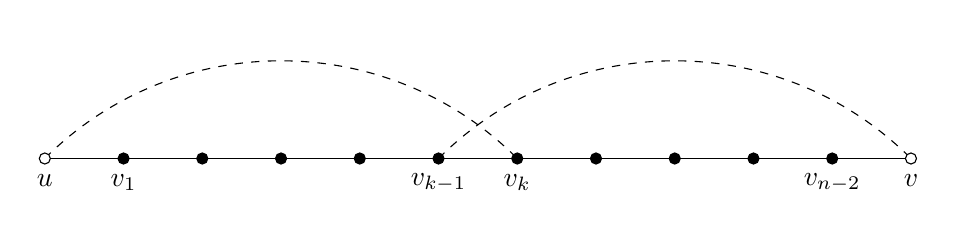
\begin{tikzpicture}
			\coordinate (a) at (-5,0);
			\coordinate (b) at (-4,0);
			\coordinate (c) at (-3,0);
			\coordinate (d) at (-2,0);
			\coordinate (e) at (-1,0);
			\coordinate (f) at (0,0);
			\coordinate (g) at (1,0);
			\coordinate (h) at (2,0);
			\coordinate (i) at (3,0);
			\coordinate (j) at (4,0);
			\coordinate (k) at (5,0);
			\coordinate (l) at (6,0);
			\draw (a) to (b) to (c) to (d) to (e) to (f) to (g) to (h) to (i) to (j) to (k) to (l);
			\draw[dashed] (a) to[bend left=45]  (g);
			\draw[dashed] (f) to[bend left=45] (l);
			\draw[fill=white] (a) circle (2pt) node[shift={(270:2ex)}] {$u\vphantom{_1}$};
			\draw[fill=black] (b) circle (2pt) node[shift={(270:2ex)}] {$v_1$};
			\draw[fill=black] (c) circle (2pt);
			\draw[fill=black] (d) circle (2pt);
			\draw[fill=black] (e) circle (2pt);
			\draw[fill=black] (f) circle (2pt) node[shift={(270:2ex)}] {$v_{k-1}$};
			\draw[fill=black] (g) circle (2pt) node[shift={(270:2ex)}] {$v_k$};
			\draw[fill=black] (h) circle (2pt);
			\draw[fill=black] (i) circle (2pt);
			\draw[fill=black] (j) circle (2pt);
			\draw[fill=black] (k) circle (2pt) node[shift={(270:2ex)}] {$v_{n-2}$};
			\draw[fill=white] (l) circle (2pt) node[shift={(270:2ex)}] {$v\vphantom{_1}$};
		\end{tikzpicture}
	\end{figure}
	
	Wenn wir ein Paar von Kanten $uv_k$ und $vv_{k-1}$ finden, dann sehen wir, dass $G$ den Hamiltonkreis $uv_kv_{k+1}\dots v_{n-2}vv_{k-1}v_{k-2}\dots v_1u$ enthält, Widerspruch! Allerdings hat $u$ in $v_2,v_3,\dots,v_{n-2}$ mindestens $\frac{n}{2}-1$ benachbarte Knoten. Das heißt, es gibt mindestens $\frac{n}{2}-1$ Knoten in $v_1,v_2,\dots, v_{n-3}$, die nicht mit $v$ benachbart sein dürfen. Dan kann $v$ jedoch höchstens $(n-2)-\parens[\big]{\frac{n}{2}-1}=\frac{n}{2}-1$ Nachbarn in $v_1,v_2,\dots, v_{n-2}$ haben. Das steht im Widerspruch zur Annahme $d(v)\geqslant \frac n2$.
\end{proof}
Das gleiche Argument zeigt, dass statt der Annahme $d(v)\geqslant \frac n2$ schon die schwächere Voraussetzung $d(u)+d(v)\geqslant n$ für alle $u,v\in V$ ausreicht. Diese Verschärfung ist als \emph{Satz von Ore} bekannt.